\begin{titre}[Fonctions de référence]

\Titre{La fonction Racine carrée}{2}
\end{titre}


 
\begin{CpsCol}
\textbf{Variations de fonctions}
\begin{description}
\item[$\square$] Connaitre la fonction Racine carrée : définition et courbes représentative.
\item[$\square$] Pour la fonction Racine carrée, résoudre graphiquement ou algébriquement une équation ou une inéquation du type $f(x) = k$, $f(x) < k$.
\end{description}
\end{CpsCol}




\begin{DefT}{Fonction Racine carrée}\index{Fonctions!Racine carrée}
La \textbf{fonction Racine carrée} $f$ est la fonction définie sur $\R^+$ par $f(x)=\sqrt x$.
\end{DefT}

 



\begin{Pp}[Variations]
\begin{minipage}{0.48\linewidth}
La fonction Racine carrée est strictement  croissante sur $\R^+$.  
\end{minipage}
\hfill
\begin{minipage}{0.48\linewidth}
\begin{tikzpicture}
\tkzTabInit[lgt=1,espcl=2]{ $x$ / 1,$f $ / 2}
{ $0$ , $+\infty$}
\tkzTabVar{-/$0$ , +/$+\infty$ }
\end{tikzpicture}
\end{minipage}
\end{Pp}

\ROC

\mini{
\EPC{1}{FR-56}{Calculer}

\EPC{1}{FR-52}{Raisonner.}

\EPC{1}{FR-54}{Calculer.}
}{
\EPC{1}{FR-53}{Chercher.}

\EPC{1}{FR-55}{Représenter.}

\EPC{1}{FR-51}{Chercher.} 
}
